Modify Program 19 (p. 82) to solve $u_{tt} = u_{xx}$ as before but with initial and boundary conditions

$$u(x,0)=0,\;\; u_x(-1,t)=0,\;\; u(1,t)=\sin(10t)$$

Produce an 'attractive' plot of the solution for $0\leq t\leq5$.\\

\begin{solution}\renewcommand{\qedsymbol}{}\ \\
    In the modification of program 19, we switch over to using the second order Chebyshev differentiation
    matrix instead of chebfft. This allowed for easier setup of the Neumann boundary condition at $x=-1$.
    After that, we also needed to define our time steps so that we could evaluate $\sin(10t)$ at the
    other boundary $x=1$. The majority of the rest of the code remained the same with some minor numeric
    changes. As such, we get the following plot, which if I do say so my self, looks attractive.
    
    \begin{center}
        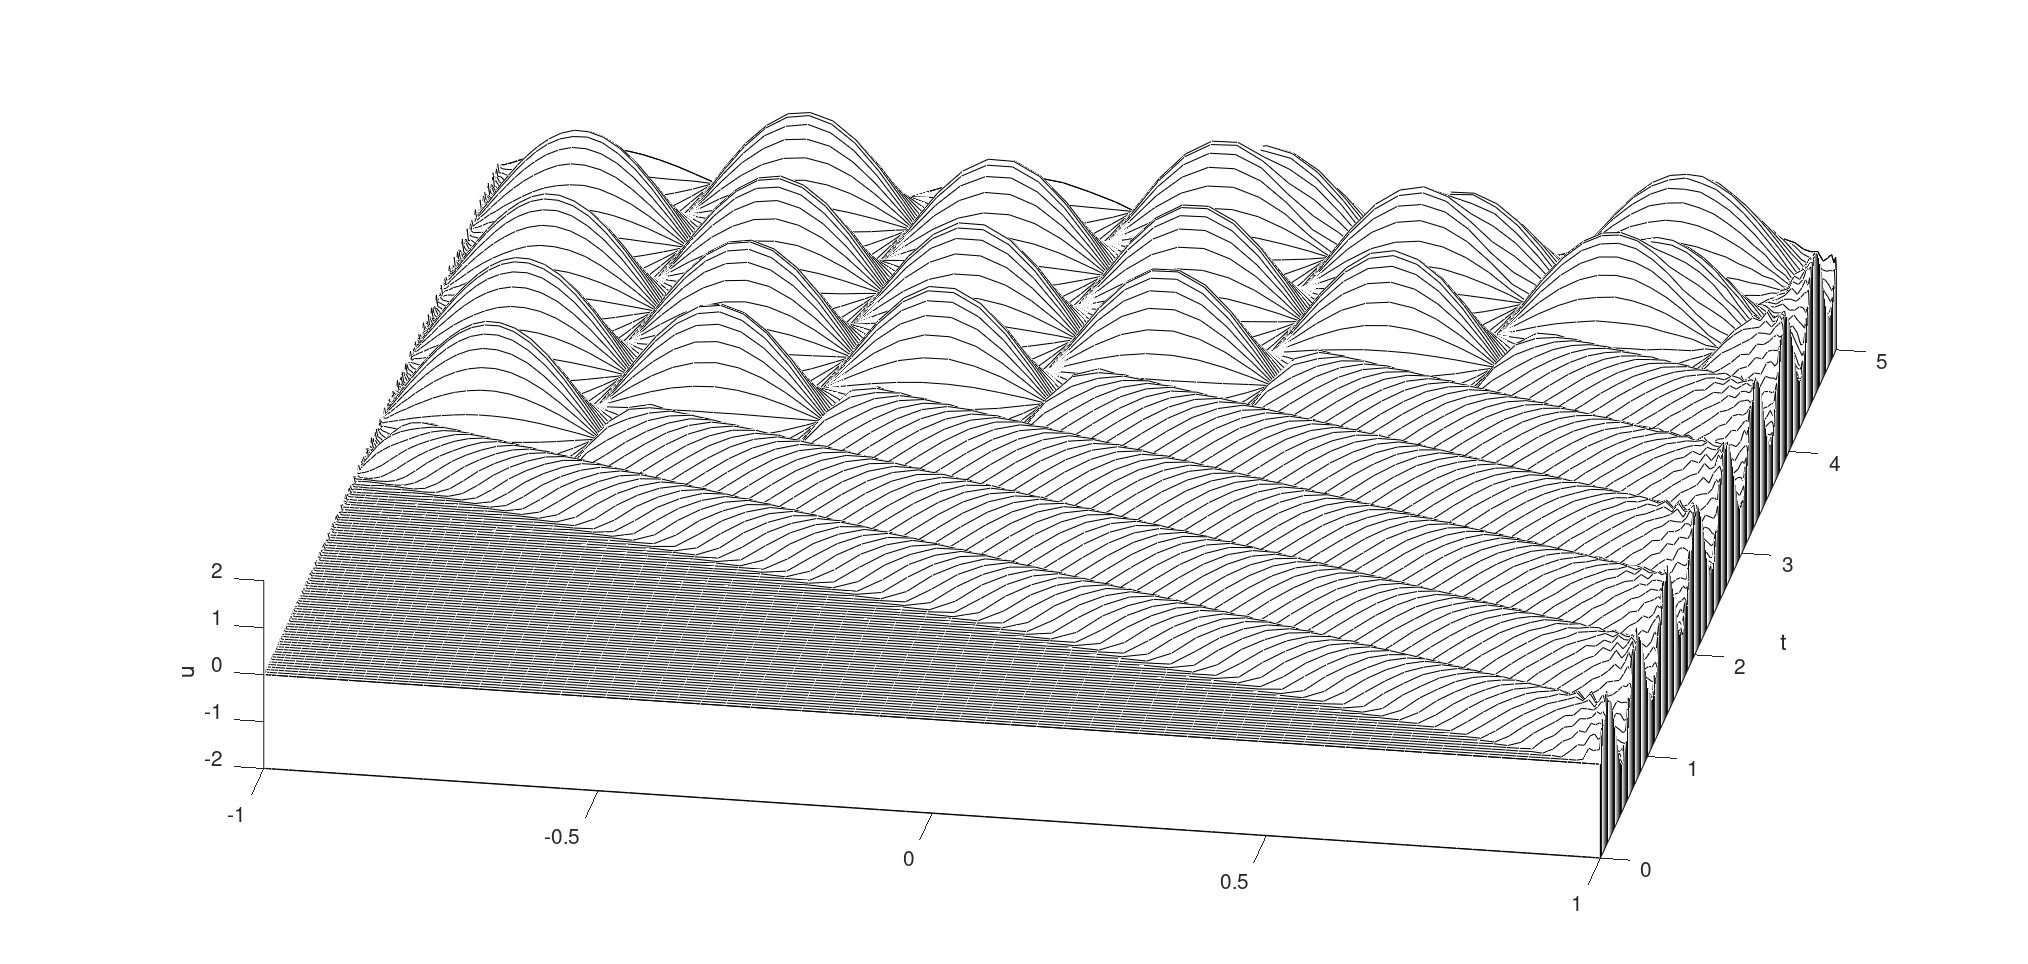
\includegraphics[scale=0.25]{problem13_3.PNG}
    \end{center}
    
\end{solution}

\newpage
\lstinputlisting{problem13_3.m}
\newpage